\section{Robust MPC}
\textbf{Uncertain constrained linear system}
\[ \boxed{x(k+1) = A x (k) + Bu(k)+w(k)\hspace{5mm} x,u \in \mathcal{X,U} \hspace{4mm}w\in \mathcal{W}}\]
\textbf{Goal:}
Design control law $u(k)= \mathcal{K}(x(k))$ such that the system: 
\begin{itemize}
    \item satisfies constraints : $\{x(k)\} \subset \mathcal{X}, \{u(k)\} \subset \mathcal{U} \forall$ disturbance realizations 
    \item Is stable: Converges to a \textbf{neighbourhood} of the origin
    \item optimizes (Expected/worst-case) "performance"
    \item Maximizes the set $\{x(0)|\textrm{Conditions 1-3 are met}\}$
\end{itemize}
\subsection{Defining a Cost to Minimize}
    Cost as a function of the disturbance seen:
    \[J(x_0,U,W) := \sum^{N-1}_{i=0} I(\Phi_i(x_0,U,W),u_i) + I_f(\Phi_N(x_0,U,W))\]
\subsection{Robust Invariance}
    \begin{minipage}{0.54\linewidth}
        Robust Positive Invariance set
        A se $\mathcal{O}^\mathcal{W}$ is said to be a robust positive invariance set for the autonomous system $x(k++) = g(x(k), w(k))$ if \[x \in \mathcal{O}^\mathcal{W} \Rightarrow g(x,w) \in \mathcal{O}^\mathcal{W} \forall w\in \mathcal{W}\]
        A set $\mathcal{O}^\mathcal{W}$ is a robust positive invariance set iff $\mathcal{O}^\mathcal{W}\subseteq \mathrm{pre}^\mathcal{W}(\mathcal{O}^\mathcal{W}$
    \end{minipage}
    \begin{minipage}{0.45\linewidth}
        \begin{center}
            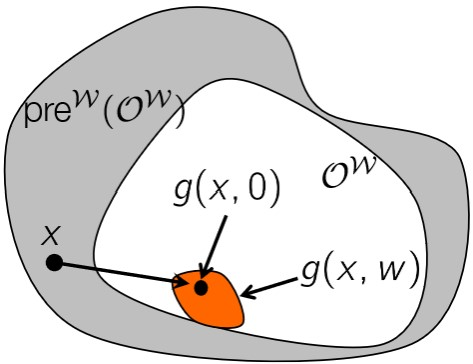
\includegraphics[width= 0.6\linewidth]{MPC_summary/Images/RPI.jpg}
        \end{center}
    \end{minipage}
    \subsubsection{Compute RPI sets}
    \textbf{Input: }$g,\mathcal{X,W}$\\
    \textbf{Output: }$\mathcal{O}^\mathcal{W}_\infty$\\
        $\hspace*{5mm} \Omega_0 \leftarrow \mathcal{X}$\\
         \hspace*{5mm}\textbf{loop}\\
         \hspace*{8mm}$\Omega_{i+1} \leftarrow \textrm{pre}^\mathcal{W}(\Omega_i) \cap\Omega_i$\\
         \hspace*{8mm}\textbf{if }$\Omega_{i+1} = \Omega_i$ \textbf{then}\\
         \hspace*{10mm}\textbf{return} $\mathcal{O} ^\mathcal{W}_\infty = \Omega_i$\\
         \hspace*{8mm}\textbf{end if}\\
         \hspace*{5mm}\textbf{end loop}\\
    \textbf{NOTE:} This is the same as for the nominal case, just $\mathrm{pre}(\Omega)$ replaced by $\mathrm{pre}^\mathcal{W}(\Omega)$
    \subsubsection{Robust Constraint Satisfaction}
    \begin{minipage}{0.22\linewidth}
        \begin{align*}
        \begin{rcases}
            \Phi_{i+1} &= A\Phi_i+Bu_i + w_i\\
            u_i &\in \mathcal{U}\\
            \Phi_i &\in \mathcal{X}\hspace{2mm}\forall W \in \mathcal{W}^N
        \end{rcases}
        \end{align*}
    \end{minipage}
    \begin{minipage}{0.6\linewidth}
         \begin{itemize}
             \item $i=0,\dots,N-1$
             \item Optimize over control action$\{u_0,\dots,u_{N-1}\}$
             \item Enforce constraints explicitly by imposing $\Phi_i\in\mathcal{X}$ and $u_i\in \mathcal{U}\forall$ sequences$W$.
         \end{itemize}
    \end{minipage}
    
     \begin{minipage}{0.22\linewidth}
        \begin{align*}
        \begin{rcases}
            \Phi_N &\in \mathcal{X}_f\\
            \Phi_{i+1} &= (A+BK)\Phi _i+w_i
        \end{rcases}
        \end{align*}
    \end{minipage}
    \begin{minipage}{0.6\linewidth}
         \begin{itemize}
             \item $i=N,\dots$
             \item Assume control law to be linear $u_i=K\Phi_i$
             \item Enforce constraints implicitly by imposing $\Phi_N$ to be in a robust invariant set $\mathcal{X}_\subseteq \mathcal{X}$ and $K\mathcal{X}_f \subseteq\mathcal{U}$ for the system $\Phi_{i+1} = (A+BK)\Phi_i+w_i$.
         \end{itemize}
    \end{minipage}
    \subsection{Set Operations}
    \textbf{Minkowski Sum:} Let $A$ and $B\subset\mathbb{R}^n$. 
    \[A\oplus B := \{x+y | x \in A,y\in B\}\]
    \textbf{Pontryagin Difference:} Let $A$ and $B\subset\mathbb{R}^n$. 
     \[A\ominus B := \{x|x+e\in A \hspace{3mm}\forall e \in B\}\]
     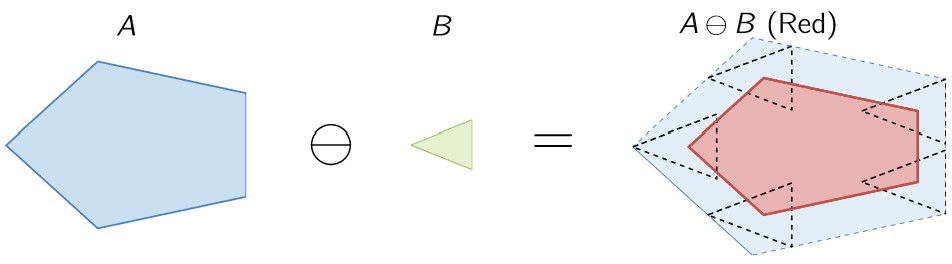
\includegraphics[width=0.9\linewidth]{MPC_summary/Images/PontryaginDiff.jpg}